\section{Experiment 9: Multi-Modal Fusion (3D CNN + Radiomics)}

\subsection{Rationale and Hypothesis}
Previous experiments highlighted the limitations of image-only deep learning models when trained on small volumetric medical datasets. Despite architectural simplifications, the high dimensionality of 3D CT data relative to the cohort size ($N=87$) remained a challenge, leading to unstable training and suboptimal generalization.

To address this issue, Experiment 9 proposes a multi-modal fusion approach that combines 3D CT imaging with radiomics features. Radiomics encode handcrafted, domain-specific descriptors of tumor intensity, texture, and shape, providing complementary high-level information. The hypothesis is that integrating these features with learned volumetric representations will improve robustness and classification performance for both \textbf{TTF-1} and \textbf{CK7}.

\subsection{Methodology}

\subsubsection{Data Preparation}
The same 87-patient dataset and stratified train--validation--test split were preserved to ensure fair comparison with previous experiments. The input pipeline was adapted to support dual modalities:
\begin{enumerate}
    \item \textbf{3D CT Volume:} Volumes were preprocessed through intensity normalization and resized to a fixed spatial resolution. Each sample was represented as a single-channel 3D tensor.
    \item \textbf{Radiomics Vector:} A vector of 107 radiomics features extracted using PyRadiomics. Features were standardized via Z-score normalization using statistics computed exclusively on the training set, preventing data leakage.
\end{enumerate}

\subsubsection{Dual-Stream Architecture}
A lightweight dual-stream neural network was implemented using a Late Fusion strategy, optimized for small datasets:

\begin{itemize}
    \item \textbf{Stream 1 (3D Image Encoder):} A compact 3D convolutional neural network composed of stacked Conv3D blocks with batch normalization and ReLU activation. Progressive max-pooling layers reduce spatial dimensionality, followed by global average pooling to obtain a dense image representation.
    \item \textbf{Stream 2 (Radiomics Encoder):} A small multi-layer perceptron (MLP) processes the radiomics features:
    \begin{itemize}
        \item Layers: $Dense(128, ReLU) \rightarrow Dropout(0.4) \rightarrow Dense(64, ReLU)$
        \item Output: A low-dimensional latent representation of radiomics features.
    \end{itemize}
    \item \textbf{Fusion Block:} The latent vectors from both streams are concatenated and passed through a shared fully connected layer with dropout and L2 regularization.
    \item \textbf{Classification Heads:} Two independent sigmoid output heads are used to perform binary classification for \textbf{TTF-1} and \textbf{CK7}.
\end{itemize}

\subsection{Experimental Results}

\subsubsection{Training Dynamics}
The model was trained using the Adam optimizer with an initial learning rate of $1 \times 10^{-4}$. Early stopping and learning rate reduction on plateau were applied based on validation loss. Compared to previous architectures, the inclusion of radiomics features led to smoother convergence and reduced sensitivity to overfitting, indicating improved training stability.

\subsubsection{Test Set Metrics}
The multi-modal model achieved its best performance using task-specific decision thresholds optimized on the validation set. On the held-out test set, the model obtained:
\begin{itemize}
    \item \textbf{TTF-1:} Accuracy = 0.67, Precision = 0.80, Recall = 0.67, F1-score = 0.73
    \item \textbf{CK7:} Accuracy = 0.89, Precision = 1.00, Recall = 0.75, F1-score = 0.86

Confusion matrix analysis shows a balanced error distribution for TTF-1 and a strong reduction in false positives for CK7, highlighting the benefit of multi-modal feature integration.( see figure 1 and figure 2)


\subsection{Conclusion of Experiment 9}
This experiment demonstrates that combining handcrafted radiomics features with learned 3D CNN representations significantly improves performance in a small-data regime. The radiomics features act as an informative prior that complements the volumetric features, enabling more reliable biomarker prediction. These findings confirm that hybrid multi-modal models are better suited than image-only deep learning approaches for limited medical imaging datasets.

    \begin{figure}[htbp]
    \centering
    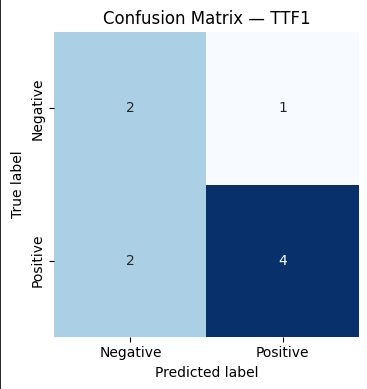
\includegraphics[width=0.6\textwidth]{ttf1.png} 
    \caption{Confusion Matrix for TTF1 (figure 1)}
    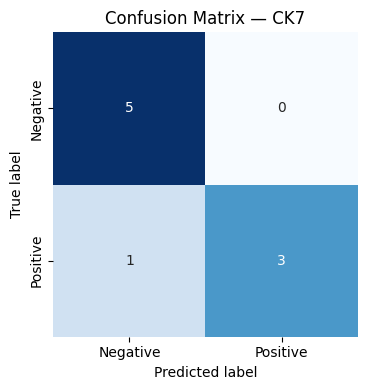
\includegraphics[width=0.6\textwidth]{ck7.png} 
    \caption{Confusion Matrix for CK7 (figure 2)}
    \label{}
    \end{figure}